\documentclass{beamer}
\usepackage[utf8]{inputenc}

\usetheme{Madrid}
\usecolortheme{default}
\usepackage{amsmath,amssymb,amsfonts,amsthm}
\usepackage{txfonts}
\usepackage{tkz-euclide}
\usepackage{listings}
\usepackage{adjustbox}
\usepackage{array}
\usepackage{tabularx}
\usepackage{gvv}
\usepackage{lmodern}
\usepackage{circuitikz}
\usepackage{tikz}
\usepackage{graphicx}

\setbeamertemplate{page number in head/foot}[totalframenumber]

\usepackage{tcolorbox}
\tcbuselibrary{minted,breakable,xparse,skins}



\definecolor{bg}{gray}{0.95}
\DeclareTCBListing{mintedbox}{O{}m!O{}}{%
  breakable=true,
  listing engine=minted,
  listing only,
  minted language=#2,
  minted style=default,
  minted options={%
    linenos,
    gobble=0,
    breaklines=true,
    breakafter=,,
    fontsize=\small,
    numbersep=8pt,
    #1},
  boxsep=0pt,
  left skip=0pt,
  right skip=0pt,
  left=25pt,
  right=0pt,
  top=3pt,
  bottom=3pt,
  arc=5pt,
  leftrule=0pt,
  rightrule=0pt,
  bottomrule=2pt,
  toprule=2pt,
  colback=bg,
  colframe=orange!70,
  enhanced,
  overlay={%
    \begin{tcbclipinterior}
    \fill[orange!20!white] (frame.south west) rectangle ([xshift=20pt]frame.north west);
    \end{tcbclipinterior}},
  #3,
}
\lstset{
    language=C,
    basicstyle=\ttfamily\small,
    keywordstyle=\color{blue},
    stringstyle=\color{orange},
    commentstyle=\color{green!60!black},
    numbers=left,
    numberstyle=\tiny\color{gray},
    breaklines=true,
    showstringspaces=false,
}
%------------------------------------------------------------

\title
{6.4.3}
\date{September 15,2025}
\author 
{AI25BTECH11003 - Bhavesh Gaikwad}



\begin{document}


\frame{\titlepage}
\begin{frame}{Question}
Find the shortest distance between the lines:\\
\begin{center}
$\vec{r} = 2\hat{i} - 5\hat{j} +\hat{k} + \lambda(3\hat{i} + 2\hat{j} + 6\hat{k})$\\
$\vec{r} = 7\hat{i} - 6\hat{k} + \mu(\hat{i} + 2\hat{j} + 2\hat{k})$
\end{center}
\end{frame}

\begin{frame}[fragile]
    \frametitle{Theoretical Solution}
Let $\vec{x}_1$ and $\vec{x}_2$ be the points on the given lines respectively.\\
$\vec{x}_1 = \myvec{2 \\ -5 \\ 1} + k_1\myvec{3 \\ 2 \\6}$ and $\vec{x}_2 = \myvec{7 \\ 0 \\ -6} + k_2\myvec{1 \\ 2 \\2}$\\
Let $\vec{A} = \myvec{2 \\ -5 \\ 1}$ and $\vec{B} = \myvec{7 \\ 0 \\ -6}$\\
Let $\vec{M} = \myvec{3 & 1 \\ 2 & 2 \\ 6 & 2}$


\begin{equation}
    (\vec{M} \, \, \vec{B}-\vec{A}) = \myvec{3 & 1 & 5 \\ 2 & 2 & 5 \\ 6 & 2 & -7}
\end{equation}
\end{frame}

\begin{frame}[fragile]
\frametitle{Theoretical Solution}
Row Transformation-1: $R_3 \rightarrow R_3 - 2R_1$
\begin{equation}
\myvec{3 & 1 & 5 \\ 2 & 2 & 5 \\ 0 & 0 & -17}
\end{equation}

Row Transformation-2: $R_2 \rightarrow R_2 - \frac{2}{3}R_1$
\begin{equation}
    \myvec{3 & 1 & 5 \\ 0 & 4/3 & 5/3 \\ 0 & 0 & -17}
\end{equation}

Therefore, The Rank is 3 $\Rightarrow$ The Lines are Skew Lines.\\

\begin{equation}
\text{Let } \vec{K} = \myvec{k_1 \\ -k_2}   
\end{equation}
\end{frame}


\begin{frame}[fragile]
\frametitle{Theoretical Solution}
\begin{equation}
    (\vec{M}^\top\vec{M})\vec{K}=\vec{M}^\top(\vec{B-A})
\end{equation}

\begin{equation}
    \myvec{49 & 19 \\ 19 & 9}\vec{K} = \myvec{-17 \\ 1}
\end{equation}

The Augmented Matrix from Equation 0.6,\\
\begin{align}
\left(
\begin{array}{cc|c}
         49 & 19 & -17 \\
         19 & 9 & 1
\end{array}
\right)
\end{align}

After Row Reductions,
\begin{align}
\left(
\begin{array}{cc|c}
         1 & 0 & -43/20 \\
         0 & 1 & 93/20
\end{array}
\right)
\end{align}

\begin{equation}
    \therefore \, \vec{K} = \myvec{-43/20 \\ 93/20}
\end{equation}
\end{frame}

\begin{frame}[fragile]
\frametitle{Theoretical Solution}
\begin{equation}
\therefore \, k_1 = -43/20 \, and \, k_2 = -93/20    
\end{equation}

From Equation 0.10,
\begin{align}
    \vec{x}_1 = \myvec{-89/20 \\ -93/10 \\ 119/10} \, and \, \vec{x}_2 =\myvec{-47/20 \\ -93/10 \\ -153/10}
\end{align}

The Minimum Distance between the given skew lines is $\norm{\vec{x}_2 - \vec{x}_2}$
\begin{equation}
    \norm{\vec{x}_2 - \vec{x}_2} = \sqrt{(\vec{x}_2 - \vec{x}_2)^\top (\vec{x}_2 - \vec{x}_2)} = \dfrac{17}{\sqrt{5}}
\end{equation}

\begin{align}
    \boxed{\text{The Minimum Distance between the given Lines =} \dfrac{17}{\sqrt{5}} \, units}
\end{align}
\end{frame}

\begin{frame}{Skew Lines}
   \centering
    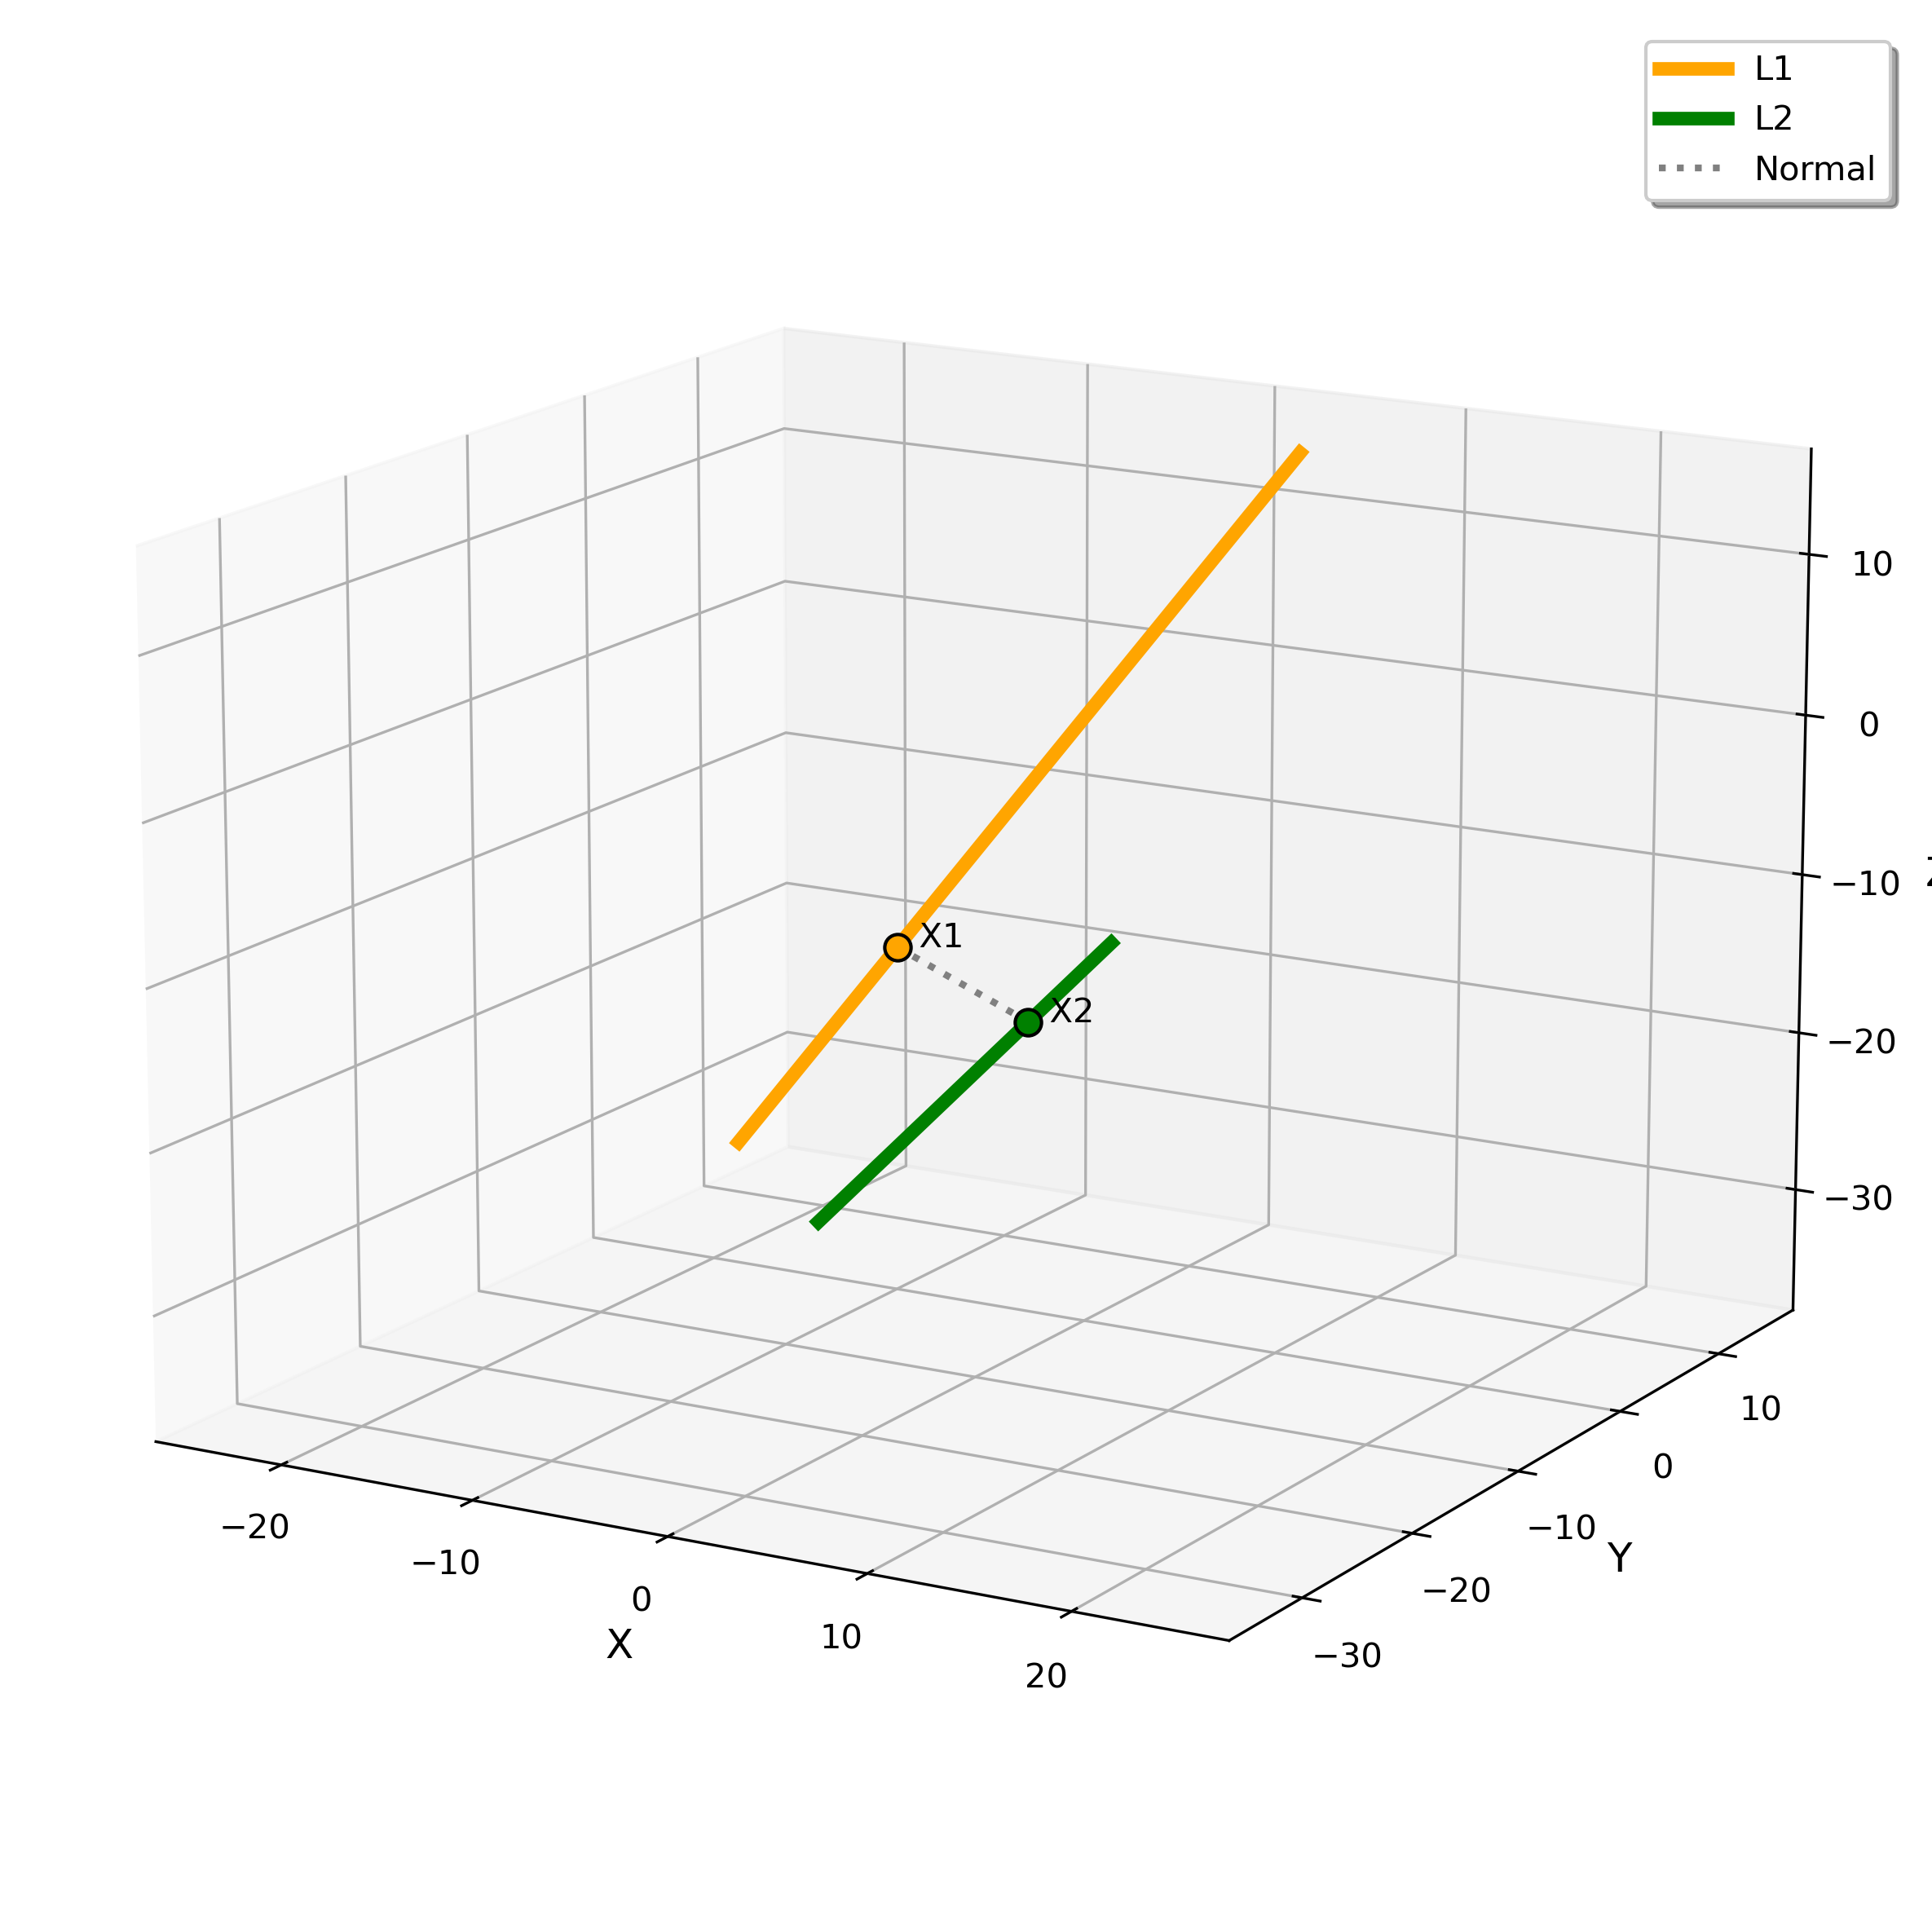
\includegraphics[width=\columnwidth, height=0.8\textheight, keepaspectratio]{figs/fig1.png}
    \label{fig:Beamer/figs/fig1.png}
\end{frame}


\end{document}